\section{Erster Entwurf}
\subsection{Entwurfsziele}
Der triviale Ansatz, die KECCAK-p-Funktion direkt in einem riesigen kombinatorischen Netz zu berechnen ist zwar theoretisch am schnellsten,
jedoch wenig platzeffizient. Da die KECCAK-p-Funktion aus 24 nahezu identischen Runden aufgebaut ist, müsste auch jede einzelne
ihrer Berechnungen nebeneinander realisiert werden. Da Ein- und Ausgabedaten mit jeweils 1600 Bits in der gleichen Größenordnung liegen
wie die Größenbeschränkung des i-Core, ist es deutlich sinnvoller, die Berechnung der Runden nacheinander über dieselbe Realisierung der Rundenfunktion durchzuführen.
Ziel dieses Entwurfs ist daher die Implementierung der Rundenfunktion in einem rein kombinatorischen Netz, womit dann in jedem Takt
jeweils eine Runde berechnet werden kann, bis schließlich die komplette KECCAK-p-Funktion berechnet ist. Die Kommunikationsschnittstelle
der Atome soll auch rudimentär implementiert werden, sodass das Einlesen und Ausgeben von Daten den dafür vorgesehenen 64-Bit Datenkanal nutzt
und die Steuerung des Atoms über maximal 6 Kontrollbits durchgeführt wird.

\subsection{Aufbau}
\begin{figure}
    \center
    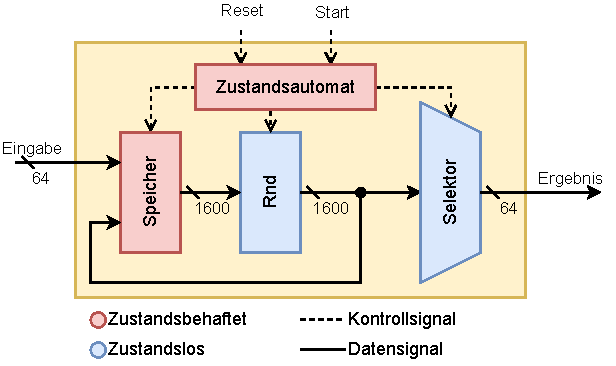
\includegraphics{images/Iteration_1.pdf}
    \caption{Aufbau des ersten Entwurfs}
    \label{fig:aufbau_iteration_1}
\end{figure}
\begin{figure}
    \center
    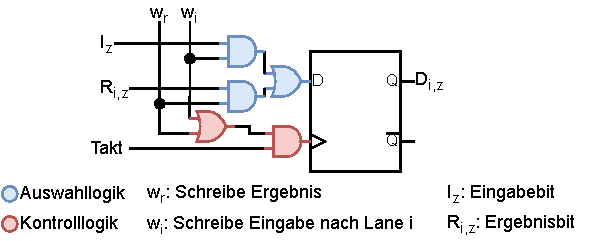
\includegraphics{images/Iteration_1_Speicher.pdf}
    \caption{Speicherzelle des ersten Entwurfs}
    \label{fig:speicher_iteration_1}
\end{figure}
In Abbildung \ref{fig:aufbau_iteration_1} ist der grobe Aufbau des Beschleunigers zu sehen. Die Rnd-Komponente berechnet aus den im Speicher liegenden Daten genau die Rundenfunktion.
Welche Runde sie berechnen soll, wird vom Zustandsautomaten bestimmt. Das Ergebnis kann nun in den Speicher zurückgeschrieben oder ausgegeben werden,
wobei der Selektor immer jeweils eine Lane des Ergebnisses an die Ausgabe anlegt. Der Zustandsautomat ist bei der Ausgabe dafür verantwortlich,
dass der Selektor alle Lanes nacheinander auswählt und somit das gesamte Ergebnis ausgibt. Der Speicher besteht aus 1600 Speicherzellen,
sodass jedes Bit der Ein-/Ausgabe der Rundenfunktion darin gespeichert werden kann. Je nachdem, ob das Ergebnis der Rundenfunktion oder die Eingabe
in den Beschleuniger übernommen werden soll, muss das entsprechende Bit ausgewählt werden. In Abbildung \ref{fig:speicher_iteration_1} ist eine Speicherzelle
mit dieser Auswahllogik skizziert. Aus einem State Array $\textbf{A}$ wird das Bit $\textbf{A}[x][y][z]$ in der Speicherzelle $D_{i,z}$ mit $i = 5 * y + x$ gespeichert.
Der Index i beschreibt also in welcher Lane, und der Index z an welcher Position innerhalb der Lane sich das Bit befindet. Die Kontrollsignale $w_i$ und $w_r$ bestimmen,
ob ein Bit aus der Eingabe ($I_z$) oder aus dem Ergebnis von Rnd ($R_{i,z}$) übernommen werden soll. In der Auswahllogik (blau) wird das entsprechende Bit ausgewählt und in der
Kontrolllogik (rot) wird am nächsten Takt der Wert in die Speicherzelle geschrieben, falls eines der beiden Bits übernommen werden soll.
Die Kontrolllogik muss dabei für jede Lane nur einmal realisiert werden, die Auswahllogik allerdings für jedes der 1600 Bits. 

\subsection{Bewertung}
Der gesamte Entwurf besteht aus 3314 LUTs. Davon werden etwa 1600 LUTs für den Datenspeicher verwendet.
Der Rest wird fast vollständig für die Berechnung der Rundenfunktion benötigt. Der Zustandsautomat und der Ergebnisselektor sind da verhältnismäßig klein.
Insgesamt ist der Entwurf damit ungefähr doppelt so groß wie es die Architektur des i-Core vorgibt. Im Folgenden wollen wir uns daher ein paar Verbesserungen anschauen,
mit denen die Größe des Beschleunigers angepasst werden kann.

\subsection{Optimierungsansätze}
\label{cha:iteration_1_optimierungen}
Eine naheliegende Möglichkeit zur Verbesserung des Platzbedarfs besteht darin den Speicheraufwand zu reduzieren, da dieser zwar viel Platz einnimmt,
aber an der Berechnung selbst nicht teilnimmt. Das Speichern der Daten außerhalb des Beschleunigers ist alleine betrachtet leider keine Option, da zur Berechnung der Rundenfunktion
ja der Gesamte Datenblock im Atom wieder vorliegen muss. Um mit weniger Daten auf einmal arbeiten zu können, muss daher zuerst die Rundenfunktion in kleinere
Teiloperationen aufgeteilt werden.

\subsubsection{Aufspalten der Rundenfunktion}
\label{cha:iteration_1_modr}
Um die Rundenfunktion in mehrere Operationen aufteilen zu können, ist eine genauere Untersuchung der Funktion selbst notwendig, um Teile ausfindig zu machen,
die unabhängig voneinander berechnet werden können. Ziel ist es, möglichst große Abschnitte in der Berechnung zu finden, die die gleiche (oder zumindest sehr ähnliche)
Operation unabhängig voneinander auf verschiedenen Daten berechnen. Diese Berechnungen können dann sequenziell statt parallel berechnet werden,
wodurch der benötige Platz reduziert wird. Damit fällt die Aufteilung in die Teilfunktionen aus der Definition der Rundenfunktion $\theta$, $\rho$, $\pi$, $\chi$ und $\iota_r$
weg, da diese Teile direkt voneinander abhängen und nicht gleichzeitig berechnet werden, sondern nacheinander.
Allerdings lassen sich alle fünf Teilfunktionen in zwei Kategorien einteilen:
\begin{enumerate}
    \item Slice-orientierte Funktionen
        Jeder Slice der Ausgabe hängt nur von einem oder zwei Slices der Eingabe ab, die anderen Slices werden ignoriert. Das sind genau die Funktionen,
        bei denen in der Definition (siehe \ref{cha:sha3_unterfunktionen}) der z-Index nicht groß verändert wird, also $\theta$, $\pi$, $\chi$ und $\iota_r$.
    \item Lane-orientierte Funktionen
        Analog handelt es sich hier um die Funktionen, bei denen jede Lane der Ausgabe nur von einer Lane der Eingabe abhängt.
        Für die Berechnung gemäß der Definition bedeutet das, dass die Indizes x und y nicht manipuliert werden.
        Zu den Lane-orientierten Funktionen zählen nur $\rho$ und $\iota_r$.
\end{enumerate}
$\iota_r$ zählt hierbei in beide Kategorien, da es sich nur um das Aufaddieren einer Konstanten handelt und somit jedes Bit der Ausgabe nur von einem Bit und einer Konstanten abhängt.
Die Rundenfunktion kann so in verschiedene Abschnitte eingeteilt werden, die nur aus Slice-orientierten oder Lane-orientierten Teilfunktionen bestehen.
Um eine möglichst gute Ausführungsgeschwindigkeit beizubehalten, ist es wichtig, die Anzahl dieser Abschnitte möglichst gering zu halten,
da so in jedem Abschnitt ein möglichst großer Teil der Berechnung durchgeführt wird. Die Rundenfunktion $Rnd_r$ besitzt drei dieser Abschnitte.
\begin{align*}
    Rnd_r & = \underbrace{\iota_r \circ \chi \circ \pi}_\text{Slice-orientiert} \circ \underbrace{\rho}_\text{Lane-orientiert} \circ \underbrace{\theta}_\text{Slice-orientiert}
\end{align*}
Für die Berechnung von KECCAK-p lässt sich die Rundenfunktion leicht modifizieren, sodass sie nur noch zwei Abschnitte besitzt.
Die Idee ist dabei, dass die Berechnung von $\theta$ jeweils an das Ende der vorherigen Runde verschoben wird.
Durch Einsetzen der Definition von $Rnd_r$ in KECCAK-p erhält man:
\begin{align*}
    \text{KECCAK-p} & = \bigcomp_{r = 0}^{23} Rnd_r = \bigcomp_{r = 0}^{23} \iota_r \circ \chi \circ \pi \circ \rho \circ \theta \\
    & = \iota_{23} \circ \chi \circ \pi \circ \rho \circ \theta \circ (\bigcomp_{r = 0}^{22} \iota_r \circ \chi \circ \pi \circ \rho \circ \theta) \\
    & = \iota_{23} \circ \chi \circ \pi \circ \rho \circ (\bigcomp_{r = 0}^{22} \theta \circ \iota_r \circ \chi \circ \pi \circ \rho) \circ \theta
\end{align*}
KECCAK-p lässt sich dann mit der modifizierten Rundenfunktion ($RMod_r$) wieder kompakt zusammenfassen:
\begin{align*}
    \alpha_r & \coloneq \iota_r \circ \chi \circ \pi \\
    \beta_r & \coloneq \theta \circ \alpha_r \\
    \gamma_r & \coloneq
    \begin{cases}
        \theta & , r = -1 \\
        \alpha_{23} & , r = 23 \\
        \beta_r & , \text{sonst}
    \end{cases} \\
    RMod_r & \coloneq 
    \begin{cases}
        \gamma_{-1} & , r = -1 \\
        \gamma_r \circ \rho & , sonst
    \end{cases} \\
    \text{KECCAK-p} & = \iota_{23} \circ \chi \circ \pi \circ \rho \circ (\bigcomp_{r = 0}^{22} \theta \circ \iota_r \circ \chi \circ \pi \circ \rho) \circ \theta \\
    & = \alpha_{23} \circ \rho \circ (\bigcomp_{r = 0}^{22} \beta_r \circ \rho) \circ \theta \\
    & = \gamma_{23} \circ \rho \circ (\bigcomp_{r = 0}^{22} \gamma_r \circ \rho) \circ \gamma_{-1} \\
    & = (\bigcomp_{r = 0}^{23} \gamma_r \circ \rho) \circ \gamma_{-1} \\
    & = \bigcomp_{i = -1}^{23} RMod_r
\end{align*}
Der Vorteil von $RMod_r$ gegenüber $Rnd_r$ ist wie anfangs motiviert, dass $RMod_r$ für jeden Index $r$ nur zwei Abschnitte mit unterschiedlicher Orientierung besitzt ($\rho$ und $\gamma$).
Da $\gamma$ eine Slice-orientierte Funktion ist, können alle Slices unabhängig voneinander nacheinander oder parallel berechnet.
Auf diese Weise ist es möglich, den von $\gamma$ benötigten Platz auf Kosten von mehr Berechnungszeit sehr stark zu reduzieren.
In Abbildung \ref{fig:gamma_berechnung} wird skizziert, wie die Berechnung von Gamma auf einzelnen Slices sehr platzeffizient implementiert werden kann, da nicht $\alpha$, $\beta$ und $\theta$
alle vollständig implementiert werden müssen. Über zwei Multiplexer können alle drei Teile berechnet werden.
\begin{figure}
    \center
    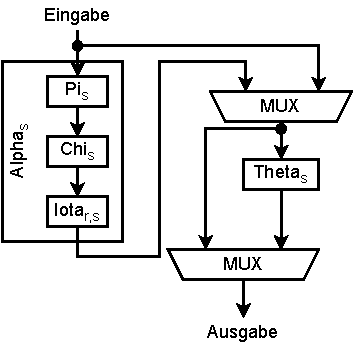
\includegraphics{images/gamma_berechnung.pdf}
    \caption{Implementierung der Gamma-Funktion}
    Die Funktionen $\pi_s$, $\chi_s$ und $\iota_{r,s}$ berechnen jeweils genau zwei Slices, sodass $\theta_s$ daraus einen Slice berechnen kann.
    \label{fig:gamma_berechnung}
\end{figure}

\subsubsection{BRAM als Datenspeicher}
Um nun den Platzbedarf des Speichers zu reduzieren, gibt es mehrere Möglichkeiten. Eine davon besteht darin, die Daten nicht in einem Flip-Flop-Register zu speichern,
sondern einen BRAM zur Speicherung von Daten zu verwenden. Leider lässt sich dieser Ansatz nicht direkt mit der Aufteilung der Rundenfunktion, wie oben beschrieben, kombinieren.
Grund dafür ist die unterschiedliche Orientierung der Operationen, die auf den Daten durchgeführt werden.
Aus einem Flip-Flop-Register können jederzeit beliebige Bits ausgelesen werden, sodass sowohl Slice- als auch Lane-orientierte Operationen direkt
aus dem Speicher mit Daten versorgt werden können. Möchte man den BRAM als Datenspeicher verwenden, so muss für den Speicher eine Orientierung festgelegt werden.
Um dann Operationen mit einer anderen Orientierung durchführen zu können, müsste jede Speicherstelle des BRAM nacheinander ausgelesen
und daraus das gewünschte Datenobjekt zusammengesetzt werden.
Daher wollen wir im zweiten Entwurf diesen Ansatz nicht verwenden, werden ihn aber im dritten Entwurf nochmal weiterverfolgen.

\subsubsection{Aufspalten des Beschleunigers}
Da ein Atom nicht ausreicht um den ganzen Datenblock zusammen mit der Rundenfunktion zu halten, kann der Beschleuniger auch in bis zu 5 Atome aufgeteilt werden,
wobei jeder Block nur noch einen Teil des Datenblocks hält und auch nur für einen Teil der Daten die modifizierte Rundenfunktion aus \ref{cha:iteration_1_modr} berechnet.
Da das Ergebnis der Rundenfunktion im Allgemeinen auch noch von den Daten anderer Blöcke abhängt, müssen diese Daten über das Interface zwischen den Atomen ausgetauscht werden.
Zwei Aspekte sind daher bei der Aufteilung wichtig:
\begin{enumerate}
    \item Wie viele Atome sind sinnvoll? Mit höherer Anzahl an Atomen nimmt die Datenmenge ab, die jedes Atom speichern muss und da jedes Atom über die Implementierung der Rundenfunktion
    verfügt, kann auch die Berechnung parallel auf den Atomen durchgeführt werden. Leider steigt mit der Anzahl der Atome auch die Menge an Datenabhängigkeiten zwischen den Atomen.
    Es gilt also herauszufinden an welchem Punkt die Kommunikationsschnittstelle zwischen den Atomen zum Bottleneck wird.
    \item Wie werden die Daten am besten auf die Atome aufgeteilt? Die Daten müssen so auf die Atome verteilt werden, dass die Datenabhängigkeiten für die Rundenfunktion möglichst gering sind.
    Jedoch sollte das Muster auch nicht zu kompliziert sein. Für die Übertragung der Daten muss ein Kommunikationsprotokoll festgelegt werden, das bestimmt,
    welche Teile der Daten in welchem Takt ausgetauscht werden. Ist das Muster zu komplex, so benötigt die Implementierung des Protokolls zu viel Platz.
\end{enumerate}
Weiterhin wäre es schön, wenn die Atome allesamt symmetrisch, also baugleich sind, es würden also alle Atome mit dem gleichen Beschleuniger konfiguriert
und über ein Kontrollsignal wird am Anfang der Ausführung bestimmt für welchen Teil der Daten ein Atom verantwortlich ist.
Dadurch ist der Beschleuniger leichter zu testen. Im Folgenden werden wir uns ein paar der naheliegenden Aufteilungsmuster anschauen.

\subsubsection{2-Block Lane-orthogonale Aufteilung}
\begin{figure}
    \center
    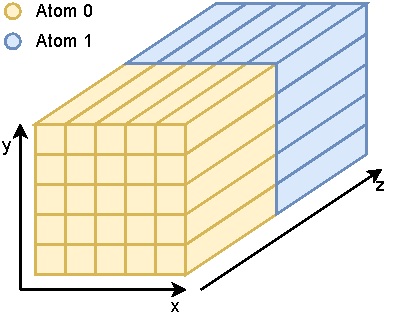
\includegraphics{images/Laneorthogonal.pdf}
    \caption{Lane-orthogonale Aufteilung des Datenblocks}
    \label{fig:2_block_laneorthogonal}
\end{figure}
Spaltet man die Daten wie in Abbildung \ref{fig:2_block_laneorthogonal} gezeigt, sodass jedes Atom jeweils 32 der insgesamt 64 Slices enthält,
so kann jedes Atom sehr einfach die Gamma-Funktion für den von ihm gehaltenen Teil berechnen. Einzig die Slices 31 und 63 müssen ausgetauscht werden,
da die Theta-Funktion für jeden Slice auch den benachbarten linken Slice benötigt. Die Berechnung der Rho-Funktion ist allerdings ein wenig komplizierter,
da jede Lane durch Rho unterschiedlich weit rotiert wird. Es muss also im Kommunikationsprotokoll für jede Lane extra festgelegt welche Bits genau in welchem
Takt ausgetauscht werden.

\subsubsection{2-Block Spalten-orthogonale Aufteilung}
\label{cha:iteration_1_optimierungen_spaltenorthogonal}
\begin{figure}
    \center
    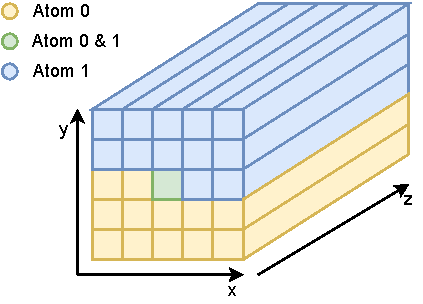
\includegraphics{images/Spaltenorthogonal.pdf}
    \caption{Spalten-orthogonale Aufteilung des Datenblocks}
    \label{fig:2_block_spaltenorthogonal}
\end{figure}
Spaltet man die Daten entlang der Lanes wie in Abbildung \ref{fig:2_block_spaltenorthogonal}, so muss für die Gamma-Funktion jeder Slice
einmal zwischen den Atomen ausgetauscht werden. Die Berechnung kann allerdings weiterhin parallel erfolgen. Auch die Rho-Funktion kann
parallel berechnet werden und benötigt keinerlei Kommunikation.

\subsubsection{Anmerkung zu Zeilen-orthogonalen Mustern}
Die Gamma-Funktion benötigt ganze Slices für die Berechnung, wenn ein Slice in einem Schritt berechnet werden soll.
Daher bestehen für Zeilen-orthogonale Aufteilungsmuster exakt die gleichen Vor- und Nachteile wie für Spalten-orthogonale Muster.
Einzig für das Ergebnis ist ein Spalten-orthogonales Muster vorteilhaft, da das Endergebnis aus den ersten 4 Lanes besteht und nur dort alle 4 Lanes in einem Atom enthalten sind.

\subsubsection{4-Block Muster}
Für die Aufteilung in 4 Blöcke können so die vorherigen Muster mehrfach angewendet oder auch miteinander kombiniert werden.
Der Speicheraufwand pro Atom sinkt hier zwar auf etwa 25\% der gesamten Datenmenge, jedoch ist der zu erwartende Gewinn an LUTs nicht mehr so groß wie beim Schritt von 1 auf 2 Atome.
Zudem steigt der Kommunikationsaufwand deutlich an, was nicht nur eine erhöhte Ausführungszeit mit sich bringt, sondern auch wieder mehr Platz im Atom benötigt.